\begin{frame}{Case Study}
  \textbf{Collaborative Intrusion Detection between Distributed Organizations}
  \begin{itemize}
    \item Each organization has its own NIDS and monitors an information system.
    \item They want to improve their detection capabilities.
    \item Share knowledge about new attacks or specific devices.
  \end{itemize}

  \pause
  \textbf{A cross-silo use case:}
  \begin{itemize}
    \item few clients (\ie, 10——100);
    \item consequent amount of data, high heterogeneity;
    \item high availability, significant computing resources.
  \end{itemize}

  \pause
  \textbf{Byzantine contributions}
  \begin{itemize}
    \item No guarantees on the quality of the contributions.
    \item Can be intentional, due to poor data quality, or due to data distribution mismatches.
  \end{itemize}
\end{frame}


\begin{frame}{Heterogeneity Headaches}
  
  \begin{columns}
    \begin{column}{.5\textwidth}
      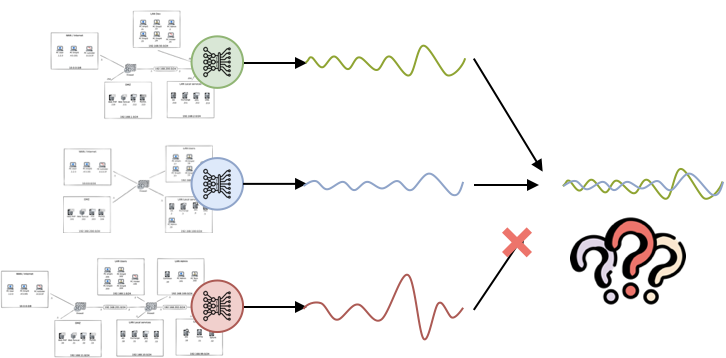
\includegraphics[width=\linewidth]{figures/intro/heterogeneity.png}
    \end{column}

    \begin{column}{.5\textwidth}

      \textcolor<2->{lightgray}{%
      \textbf{Challenge I}: \textit{Too much heterogeneity leads to poor performance\dots}
      }
      \only<1>{%
        \begin{itemize} \small
          \item How to handle different feature sets, data distributions?
          \item How to consider models that are dissimilar because they "contain" relevant knowledge?
        \end{itemize}
      }
      \vspace{1ex}


      \textcolor<1>{lightgray}{%
      \textbf{Challenge II}: \textit{Difficult to identify malicious contributions when models are different\dots}
      }
      
      \only<2>{%
        \begin{itemize} \small
          \item Are model "dissimilar" because they are different, or because they are malicious/poisoned?
        \end{itemize}
      }
      \vspace{1ex}
      
    \end{column}
  \end{columns}  
\end{frame}

\begin{frame}{Problem Statement}
  \begin{block}{Quality Assessment in Heterogeneous Settings}
    For $n$ participants $p_i$ and their local datasets $d_i$ of unknown similarity, each participant uploads a model update $w_i^r$ at each round $r$. Given $P = \{ p_1, p_2, \dots, p_n \} $ and $W = \{ w_1^r, w_2^r, \dots, w_n^r \} $, how can one assess the quality of each participant’s contribution without making assumptions on the data distribution across the datasets $d_i$?
  \end{block}
\end{frame}

\begin{frame}{Outline}
  \centering
  \begin{minipage}[t]{.8\textwidth}
    \tableofcontents%[hideallsubsections,]
  \end{minipage}
\end{frame}

